\FloatBarrier
\appendix
\section{Transport identity and curvature}
\label{app:transport}
For fixed $w$, the loss $\ell_w(r)=-w^\top r$ is $\lVert w\rVert_2$-Lipschitz. The positive-part CVaR representation gives the upper bound
\begin{equation}
\CVaR^Q_\alpha(\ell_w)\leq
\CVaR^{\widehat P_N}_\alpha(\ell_w)+\frac{\epsilon\lVert w\rVert_2}{1-\alpha}
\end{equation}
whenever $W_1(Q,\widehat P_N)\leq\epsilon$. To attain it on unrestricted support, select exactly $q=1-\alpha$ mass from the largest nominal losses, splitting boundary atoms if necessary. For $w\ne0$, move this mass in return space by
\begin{equation}
-\frac{\epsilon}{q}\frac{w}{\lVert w\rVert_2}.
\end{equation}
The transport plan costs $\epsilon$, increases each selected loss by $\epsilon\lVert w\rVert_2/q$, and preserves its position in the upper tail. Its tail average attains the upper bound. For $w=0$ both sides vanish. This specializes established Wasserstein risk reformulations \cite{esfahani,kuhntutorial}; it is not a new theorem. Atom splitting also explains why empirical ES averages fractional boundary mass when $Nq$ is noninteger.

Equation~\eqref{eq:allocation} retains nominal mean return. If one instead robustifies mean minus $\gamma$ times CVaR under the \emph{same} adverse law, this transport also lowers the mean by $\epsilon\lVert w\rVert_2$. The penalty becomes $\epsilon\lVert w\rVert_2[1+\gamma/(1-\alpha)]$. That alternative is not the implemented objective. Support constraints require a new derivation.

The covariance ridge makes $\Omega_t$ positive definite for the nondegenerate scenario samples used here. For $\lambda>0$, $-\lambda w^\top\Omega_t w/2$ is strictly concave. The remaining terms in \eqref{eq:allocation} are concave, so the objective is strictly concave on the convex feasible set and has a unique maximizer. Uniqueness does not imply strictly positive components. Actual multi-asset holdings are an empirical result, reported separately from this mathematical property.

\section{Additional forecast diagnostics}
\label{app:forecast}
\begin{table*}[t]
\centering\small\setlength{\tabcolsep}{5pt}
\caption{Additional forecast diagnostics. MAE concerns log next-day rolling volatility. F-QLIKE concerns annualized future five-day squared-return variation on nonoverlapping target windows. Lower is better. This separate future target was not the training objective and is not observed latent variance.}
\label{tab:additional_forecast}
\begin{tabular}{llrrrrrr}\toprule
& &\multicolumn{2}{c}{Persistence}&\multicolumn{2}{c}{Window update}&\multicolumn{2}{c}{Gated residual}\\
\cmidrule(lr){3-4}\cmidrule(lr){5-6}\cmidrule(lr){7-8}
ETF&Period&MAE&F-QLIKE&MAE&F-QLIKE&MAE&F-QLIKE\\\midrule
SPY & 2019--24 & 0.0386 & 0.6032 & 0.0281 & 0.5976 & 0.0349 & 0.5565 \\
SPY & 2025 & 0.0414 & 0.7706 & 0.0289 & 0.7563 & 0.0334 & 0.7176 \\
IWM & 2019--24 & 0.0355 & 0.4593 & 0.0259 & 0.4637 & 0.0305 & 0.4475 \\
IWM & 2025 & 0.0370 & 0.4767 & 0.0265 & 0.4677 & 0.0288 & 0.4511 \\
TLT & 2019--24 & 0.0333 & 0.3682 & 0.0250 & 0.3849 & 0.0286 & 0.3673 \\
TLT & 2025 & 0.0358 & 0.2525 & 0.0245 & 0.2580 & 0.0262 & 0.2527 \\
GLD & 2019--24 & 0.0374 & 0.4780 & 0.0281 & 0.4853 & 0.0317 & 0.4698 \\
GLD & 2025 & 0.0416 & 0.6057 & 0.0293 & 0.5845 & 0.0332 & 0.5482
\\\bottomrule
\end{tabular}
\end{table*}
Table~\ref{tab:additional_forecast} distinguishes the smoothed target from future variation. Residual forecasts have lower displayed future QLIKE than persistence in seven of eight asset--period comparisons; TLT in 2025 is slightly worse. These point estimates do not supply an inference about true latent variance. All model-level RMSE, MAE, rolling-proxy QLIKE, annual seed errors, and paired loss-difference intervals are retained in the companion CSV files, including the EWMA and HAR-type comparators.

\section{Annual parameter estimates}
\label{app:parameters}
\begin{table*}[t]
\centering\footnotesize\setlength{\tabcolsep}{5pt}
\caption{All annual physical-model fits, displayed to two significant figures. LL gain is fitted minus fixed-reference total log likelihood on the same 756 fitting returns. MC SD is fitted likelihood variation across five 4,096-particle seeds. Neither is a parameter uncertainty interval. Data-dependent starting values, the fixed reference, and fitted candidates are compared by training likelihood only.}
\label{tab:all_parameters}
\begin{tabular}{llrrrrrr}\toprule
ETF&Test year&$\kappa$&$\theta$&$\xi$&$\rho$&LL gain&MC SD\\\midrule
SPY & 2019 & 11 & 0.015 & 0.46 & -0.54 & 12.31 & 0.34 \\
SPY & 2020 & 9.9 & 0.014 & 0.44 & -0.71 & 16.77 & 0.35 \\
SPY & 2021 & 6.4 & 0.056 & 0.72 & -0.60 & 31.63 & 0.21 \\
SPY & 2022 & 10 & 0.032 & 0.71 & -0.67 & 37.09 & 0.75 \\
SPY & 2023 & 7.7 & 0.053 & 0.78 & -0.74 & 31.05 & 0.41 \\
SPY & 2024 & 8.6 & 0.031 & 0.55 & -0.78 & 5.29 & 0.21 \\
SPY & 2025 & 7.3 & 0.031 & 0.46 & -0.84 & 3.55 & 0.16 \\
IWM & 2019 & 8.2 & 0.027 & 0.41 & -0.71 & 1.16 & 0.12 \\
IWM & 2020 & 11 & 0.022 & 0.44 & -0.78 & 6.34 & 0.18 \\
IWM & 2021 & 4.9 & 0.058 & 0.68 & -0.62 & 23.88 & 0.24 \\
IWM & 2022 & 5.4 & 0.070 & 0.82 & -0.67 & 30.82 & 0.56 \\
IWM & 2023 & 8.0 & 0.093 & 0.93 & -0.70 & 32.26 & 0.32 \\
IWM & 2024 & 6.5 & 0.056 & 0.36 & -0.58 & 3.37 & 0.14 \\
IWM & 2025 & 4.4 & 0.054 & 0.28 & -0.49 & 3.51 & 0.066 \\
TLT & 2019 & 0.63 & 0.011 & 0.046 & 0.57 & 36.98 & 0.079 \\
TLT & 2020 & 0.73 & 0.012 & 0.071 & 0.79 & 46.83 & 0.15 \\
TLT & 2021 & 11 & 0.019 & 0.43 & 0.14 & 45.02 & 0.47 \\
TLT & 2022 & 14 & 0.023 & 0.51 & 0.079 & 38.29 & 1.2 \\
TLT & 2023 & 9.2 & 0.039 & 0.53 & -0.046 & 26.27 & 0.35 \\
TLT & 2024 & 1.3 & 0.037 & 0.12 & -0.50 & 6.43 & 0.15 \\
TLT & 2025 & 0.82 & 0.032 & 0.11 & -0.85 & 10.34 & 0.091 \\
GLD & 2019 & 2.1 & 0.013 & 0.096 & 0.31 & 32.23 & 0.13 \\
GLD & 2020 & 11 & 0.011 & 0.18 & 0.50 & 45.26 & 0.086 \\
GLD & 2021 & 16 & 0.018 & 0.51 & 0.25 & 48.26 & 0.23 \\
GLD & 2022 & 19 & 0.023 & 0.71 & 0.14 & 45.86 & 0.32 \\
GLD & 2023 & 25 & 0.026 & 0.69 & 0.038 & 38.94 & 0.18 \\
GLD & 2024 & 27 & 0.020 & 0.51 & 0.14 & 27.61 & 0.15 \\
GLD & 2025 & 23 & 0.022 & 0.44 & 0.53 & 33.13 & 0.10
\\\bottomrule
\end{tabular}
\end{table*}
\begin{figure*}[t]
\centering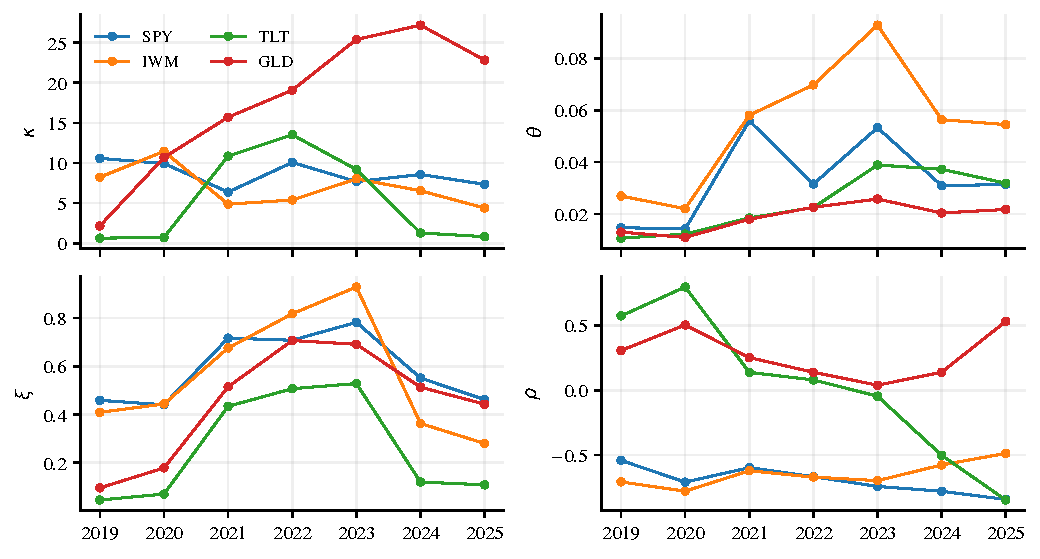
\includegraphics[width=\textwidth]{figures/study_calibration.pdf}
\caption{Annual asset-specific estimates available before each evaluation year. Changes reflect rolling historical samples and approximate bounded estimation, rather than parameter changes inferred from the later evaluation outcomes.}
\label{fig:parameters}
\end{figure*}
Table~\ref{tab:all_parameters} and Figure~\ref{fig:parameters} make the annual estimates explicit. All refinement stages meet their numerical stopping condition. Five selected fits retain an archived likelihood-based start when its five-seed checking score exceeds the other candidates. Thus tighter searches do not imply that every selected coordinate has moved away from a line-search trial value. Finite-particle irregularity and identification limitations remain, and two significant figures are used throughout the parameter tables. Full computational values, starts, search statuses, likelihood evaluations, Feller gaps, and causal fit dates are archived.

\section{Sensitivity and simulation checks}
\label{app:sensitivity}
\begin{table*}[t]
\centering\small\setlength{\tabcolsep}{5pt}
\caption{Declared 2,000-scenario sensitivities, evaluated on 2025 calendar returns after recomputing complete paths from 2019. Radius values are vector simple-return distances; costs are fractions of risky turnover. CAGR and daily ES are percentages. Other coefficients retain their primary settings.}
\label{tab:sensitivity}
\begin{tabular}{lllr rr}\toprule
Setting&Value&Strategy&CAGR&ES&$N_{\rm eff}$\\\midrule
epsilon & 0 & Fixed-radius DRO & 45.83 & 1.87 & 1.88 \\
epsilon & 5e-05 & Fixed-radius DRO & 45.90 & 1.87 & 1.89 \\
epsilon & 0.0001 & Fixed-radius DRO & 46.02 & 1.87 & 1.90 \\
epsilon & 0.00025 & Fixed-radius DRO & 46.62 & 1.87 & 1.92 \\
epsilon & 0.0005 & Fixed-radius DRO & 46.44 & 1.88 & 1.95 \\
lambda & 0 & Fixed-radius DRO & 47.88 & 2.05 & 1.80 \\
lambda & 1 & Fixed-radius DRO & 46.99 & 2.01 & 1.83 \\
lambda & 4 & Fixed-radius DRO & 46.02 & 1.87 & 1.90 \\
lambda & 10 & Fixed-radius DRO & 43.37 & 1.74 & 1.98 \\
cost & 0 & Fitted Heston / residual & 54.27 & 1.72 & 1.82 \\
cost & 0 & Fixed-radius DRO & 53.67 & 1.71 & 1.83 \\
cost & 0 & Adaptive-radius DRO & 53.06 & 1.69 & 1.85 \\
cost & 0.0007 & Fitted Heston / residual & 45.83 & 1.87 & 1.88 \\
cost & 0.0007 & Fixed-radius DRO & 46.02 & 1.87 & 1.90 \\
cost & 0.0007 & Adaptive-radius DRO & 46.45 & 1.85 & 1.93 \\
cost & 0.0014 & Fitted Heston / residual & 38.29 & 2.01 & 1.93 \\
cost & 0.0014 & Fixed-radius DRO & 38.38 & 2.00 & 1.94 \\
cost & 0.0014 & Adaptive-radius DRO & 38.58 & 1.97 & 1.97
\\\bottomrule
\end{tabular}
\end{table*}
\begin{table*}[t]
\centering\small\setlength{\tabcolsep}{5pt}
\caption{Conditional 2025 allocation checks at 2,000 and 20,000 scenarios under independent draws. Distance is adaptive-DRO weight $L^1$ distance from seed zero at the same scenario count; tilt is its distance from matched nominal allocation under the same draws. Every check uses common pretrade weights reconstructed from the primary 20,000-scenario nominal path. These are allocation diagnostics, separate from the full backtests.}
\label{tab:monte_carlo}
\begin{tabular}{rrrrr}\toprule
Scenarios&Seed offset&Mean distance&95th percentile&Mean robustness tilt\\\midrule
2000 & 0 & 0.0000 & 0.0000 & 0.0112 \\
2000 & 10000 & 0.0224 & 0.1225 & 0.0119 \\
2000 & 20000 & 0.0225 & 0.1126 & 0.0123 \\
20000 & 0 & 0.0000 & 0.0000 & 0.0128 \\
20000 & 10000 & 0.0053 & 0.0236 & 0.0134 \\
20000 & 20000 & 0.0059 & 0.0285 & 0.0130
\\\bottomrule
\end{tabular}
\end{table*}
The sensitivity grid is descriptive; it is not a search for a preferred test-period coefficient. Higher fees change the optimizer's trading decisions as well as realized deductions. The $\lambda=0$ row removes the quadratic term while retaining multivariate CVaR, costs, and the fixed-radius norm penalty. Such a multivariate problem is not subject to the original single-exposure endpoint argument.

At 2,000 scenarios, mean independent-seed allocation distances of about 0.022 exceed robustness tilts near 0.012. At 20,000 scenarios, mean distances decrease to about 0.005--0.006, while tilts remain near 0.013. Both counts use their own first-seed reference and identical pretrade weights, so this reduction is not measured against a noisy lower-count reference. Some dates remain sensitive, as the 95th-percentile distances show. Three seeds characterize numerical variation rather than establish an asymptotic convergence rate.

\begin{table*}[t]
\centering\small\setlength{\tabcolsep}{6pt}
\caption{Full-path 20,000-scenario seed sensitivity. CAGRs and annualized arithmetic mean-return differences are percentages; ES differences are daily basis points. Every difference is adaptive DRO minus matched nominal allocation. Complete paired intervals for every seed are public.}
\label{tab:paired_seeds}
\begin{tabular}{rlrrrr}\toprule
Seed offset&Period&Nominal CAGR&Adaptive CAGR&Mean diff.&ES diff.\\\midrule
0 & 2019--24 & 11.20 & 11.21 & 0.003 & -0.81 \\
0 & 2025 & 44.06 & 44.59 & 0.353 & -3.02 \\
10000 & 2019--24 & 11.16 & 11.18 & 0.013 & -0.86 \\
10000 & 2025 & 43.89 & 44.02 & 0.075 & -3.22 \\
20000 & 2019--24 & 11.22 & 11.27 & 0.040 & -0.97 \\
20000 & 2025 & 43.59 & 43.94 & 0.235 & -2.39
\\\bottomrule
\end{tabular}
\end{table*}
The three full backtests use independent simulator draws for the whole 2019--2025 path. No holdings restart at the confirmation boundary. Table~\ref{tab:paired_seeds} displays their variation without choosing the most favorable seed. Mean-return intervals include zero in every comparison.

\section{Reproduction and validation}
\label{app:reproduction}
The versioned public release contains executable code, a design protocol, input hashes and source URLs, trained model checkpoints, annual fit records, and aggregate diagnostics. Provider observations and date-by-date experimental caches are excluded. A reader with appropriate data access can download local inputs, verify their canonical hashes, reconstruct neural predictions with \texttt{forecast.py --reuse-checkpoints}, rebuild latent-state paths with \texttt{calibrate.py}, and run \texttt{portfolio.py}, \texttt{paired\_accuracy.py}, \texttt{analyze.py}, \texttt{analyze\_accuracy.py}, \texttt{extra\_checks.py}, and \texttt{paper\_assets.py}. The README distinguishes exact matching-input replication from a current-provider-data rerun. Public summaries suffice to regenerate the numerical tables and the forecast/parameter figures; wealth and allocation figures require regenerated local paths.

Ten mathematical and timing tests pass. Nine cover the persistence identity, fractional-mass ES versus an independent linear program, explicit multivariate tail transport, a known quadratic portfolio solution, CVaR versus an independent program, deterministic-variance Gaussian filtering, leverage-conditioned variance means, causal dates, and portfolio feasibility/common holding intervals. A tenth compares the tail-separation solver with the full empirical conic epigraph, including fractional tail mass and cash-enabled cases. Checkpoint replay reconstructs all saved forecasts to numerical precision, and all 28 validation gates are independently checked.

The primary paired experiment contains 3,159 portfolio solves. Sixty-two final statuses are \texttt{optimal\_inaccurate}; every solution nevertheless passes the recorded primal feasibility and full-scenario tail-separation checks, with maximum violations below $2\times10^{-10}$ and tail-objective underestimation below $10^{-10}$. These diagnostics do not turn an approximate solver status into a formal exact-arithmetic certificate. As an additional check, eight independent full-epigraph solves on four fixed schedule positions with 20,000 scenarios differ in objective by at most $1.2\times10^{-10}$ and in weight $L^1$ distance by at most $1.1\times10^{-4}$. The dates and differences are public. These checks validate computational behavior, not market generalization.
